\subsection{实验目的-配置 iptables 按网段访问 ftp 服务}
通过配置 iptables 防火墙来按网段访问 ftp 服务.
%
\subsection{实验原理}
Iptables 防火墙在做信息包过滤决定时,有一套遵循和组成的规则,这些规
则存储在专用的信息包过滤表中,而这些表集成在 Linux 内核中。在信息包过滤
表中,规则被分组放在我们所谓的链(chain)中。而 \texttt{netfilter/iptables} IP
信息包过滤系统是一款功能强大的工具,可用于添加、编辑和移除规则。
%
\subsection{实验环境}
操作系统:
\begin{itemize}
  \item Windows 7
  \item Windows server 2003
  \item CentOS 6.5
  \item CentOS 6.5
\end{itemize}
%
\subsection{实验步骤}
\subsubsection{在当前环境下内外网均可连接 ftp 服务}
打开 Windows 7 的 cmd,
输入
\begin{minted}[bgcolor=bg,breaklines=true]{sh}
ftp 10.0.0.2
\end{minted}
输入用户名 \texttt{ftp},密码 \texttt{123456},登录成功。
\begin{figure}[H]
  \begin{center}
    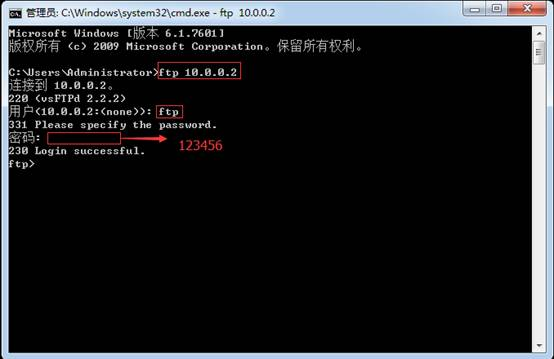
\includegraphics[width=0.40\textwidth]{2_7_1.jpeg}
  \end{center}
\end{figure}

打开 Windows server 2003 的 cmd,
输入
\begin{minted}[bgcolor=bg,breaklines=true]{sh}
ftp 10.0.0.2
\end{minted}
输入用户名 \texttt{ftp},
密码 \texttt{123456},登录成功。
\begin{figure}[H]
  \begin{center}
    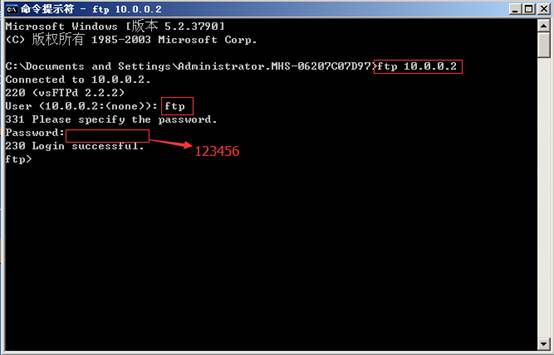
\includegraphics[width=0.40\textwidth]{2_7_2.jpeg}
  \end{center}
\end{figure}
%
\subsubsection{配置 iptables,按网段访问 ftp 服务}
这里以 Windows server 2003 能够访问 ftp 服务,
而 Windows 7 不能访问 ftp 服务为例.

在防火墙 CentOS 6.5 的终端输入如下命令,清空防火墙规则。
\begin{minted}[bgcolor=bg,breaklines=true]{sh}
iptables -F
iptables -X
iptables -Z
iptables -L -n --line-numbers
\end{minted}
\begin{figure}[H]
  \begin{center}
    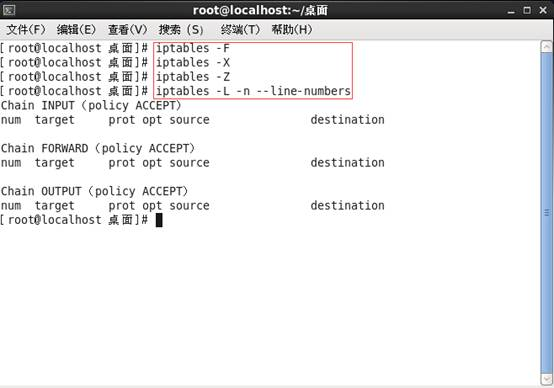
\includegraphics[width=0.40\textwidth]{2_7_3.jpeg}
  \end{center}
\end{figure}

配置防火墙,按网段访问 ftp 服务。在终输入如下命令,在转发的数据包
中,如果源地址为 \texttt{192.168.1.0/24},
目标端口为 21,则将该数据包丢弃,同时
允许源地址为 \texttt{20.0.0.2/24},
目标端口为 21 的数据包通过,这一条防火墙规则可加可不加。
\begin{minted}[bgcolor=bg,breaklines=true]{sh}
iptables -t filter -A FORWARD -s 192.168.1.0/24 -p tcp --dport 21 -j DROP
iptables -t filter -A FORWARD -s 20.0.0.0/24 -p tcp --dport 21 -j ACCEPT
/etc/init.d/iptables save
/etc/init.d/iptables restart
cat /etc/sysconfig/iptables
\end{minted}
\begin{figure}[H]
  \begin{center}
    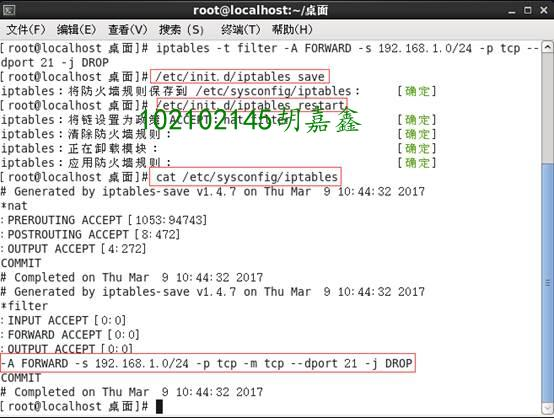
\includegraphics[width=0.40\textwidth]{2_7_4.jpeg}
  \end{center}
\end{figure}

此时在 Windows 7 的 cmd 上,
输入
\begin{minted}[bgcolor=bg,breaklines=true]{sh}
ftp 10.0.0.2
\end{minted}
已经不能连接 ftp 服务了。
\begin{figure}[H]
  \begin{center}
    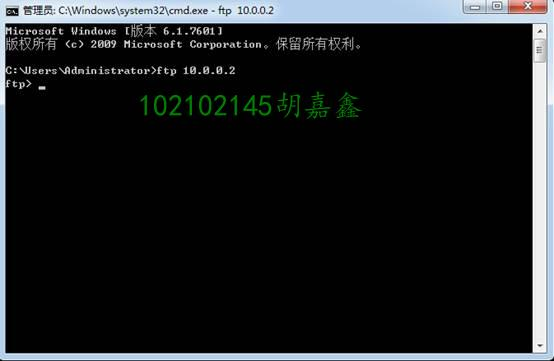
\includegraphics[width=0.40\textwidth]{2_7_5.jpeg}
  \end{center}
\end{figure}

但在 Windows server 2003 的 cmd 上,
输入
\begin{minted}[bgcolor=bg,breaklines=true]{sh}
ftp 10.0.0.2
\end{minted}
可以继续连接 ftp 服务。
\begin{figure}[H]
  \begin{center}
    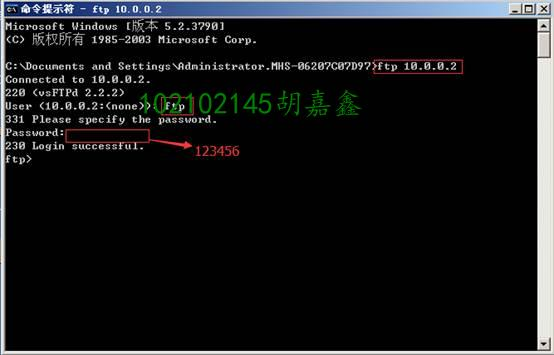
\includegraphics[width=0.40\textwidth]{2_7_6.jpeg}
  \end{center}
\end{figure}
%
